\documentclass[11pt]{ctexart}
\usepackage[top=2cm, bottom=2cm, left=2cm, right=2cm]{geometry}
\usepackage{algorithm}
\usepackage{algorithmicx}
\usepackage{algpseudocode}
\usepackage{amsmath}
\usepackage{graphicx}
\usepackage{listings}
\usepackage{xcolor}
\usepackage{float}
\usepackage{amsmath}
\usepackage{amssymb}
\usepackage{listings} %插入代码
\usepackage{xcolor} %代码高亮

\floatname{algorithm}{算法}
\renewcommand{\algorithmicrequire}{\textbf{输入:}}
\renewcommand{\algorithmicensure}{\textbf{输出:}}



\lstset{numbers=left, %设置行号位置
        numberstyle=\tiny, %设置行号大小
        keywordstyle=\color{blue}, %设置关键字颜色
        commentstyle=\color[cmyk]{1,0,1,0}, %设置注释颜色
        frame=single, %设置边框格式
        escapeinside=``, %逃逸字符(1左面的键),用于显示中文
        breaklines, %自动折行
        extendedchars=false, %解决代码跨页时,章节标题,页眉等汉字不显示的问题
        xleftmargin=2em,xrightmargin=2em, aboveskip=1em, %设置边距
        tabsize=4, %设置tab空格数
        showspaces=false %不显示空格
}

\title{\huge\bf
算法设计大作业(一)}
\author{毛圆鑫 - 201721012271}
\date{Oct 25, 2019}

\begin{document}
\maketitle
\section*{说明}
\noindent 这是算法设计课的第一个大作业,我完成的题目是\textbf{CCF - 201612-4}\\
大家可以在http://118.190.20.162/home.page这个网址中获取到题目和测试集\\
当然,下面也有完整的题目与分析报告,整篇文档是基于latex语言设计的\\
源码见附件或github.com/punk-boy/algorithm/algorithm.tex\\


\section{题目描述}
\noindent\textbf{问题描述}\\
  给定一段文字,已知单词$a_{1}$, $a_{2}$, $\dots$, $a_{n}$出现的频率分别$t_{1}$, $t_{2}$, $\dots$, $t_{n}$。可以用01串给这些单词编码,即将每个单词与一个01串对应,使得任何一个单词的编码(对应的01串)不是另一个单词编码的前缀,这种编码称为前缀码。\\
  使用前缀码编码一段文字是指将这段文字中的每个单词依次对应到其编码。一段文字经过前缀编码后的长度为:\\
  $L=a_{1}$的编码长度$\times t_{1}+a_{2}$的编码长度$\times t_{2}+ \dots + a_{n}$的编码长度$\times t_{n}$。\\
  定义一个前缀编码为字典序编码,指对于$1\leqslant i < n$,ai的编码(对应的01串)的字典序在$a_{i}$+1编码之前,即$a_{1}$, $a_{2}$, $\dots$, $a_{n}$的编码是按字典序升序排列的。\\
  例如,文字E A E C D E B C C E C B D B E中, 5个单词A、B、C、D、E出现的频率分别为1, 3, 4, 2, 5,则一种可行的编码方案是A:000, B:001, C:01, D:10, E:11,对应的编码后的01串为1100011011011001010111010011000111,对应的长度L为3×1+3×3+2×4+2×2+2×5=34。\\
  在这个例子中,如果使用哈夫曼(Huffman)编码,对应的编码方案是A:000, B:01, C:10, D:001, E:11,虽然最终文字编码后的总长度只有33,但是这个编码不满足字典序编码的性质,比如C的编码的字典序不在D的编码之前。\\
  在这个例子中,有些人可能会想的另一个字典序编码是A:000, B:001, C:010, D:011, E:1,编码后的文字长度为35。\\
  请找出一个字典序编码,使得文字经过编码后的长度L最小。在输出时,你只需要输出最小的长度L,而不需要输出具体的方案。在上面的例子中,最小的长度L为34。\\
\textbf{输入格式}\\
  输入的第一行包含一个整数n,表示单词的数量。\\
  第二行包含n个整数,用空格分隔,分别表示$a_{1}$, $a_{2}$, $\dots$, $a_{n}$出现的频率,即$t_{1}$, $t_{2}$, $\dots$, $t_{n}$。请注意$a_{1}$, $a_{2}$, $\dots$, $a_{n}$具体是什么单词并不影响本题的解,所以没有输入$a_{1}$, $a_{2}$, $\dots$, $a_{n}$。\\
\textbf{输出格式}\\
  输出一个整数,表示文字经过编码后的长度$L$的最小值。\\
\textbf{样例输入}\\
  5\\
  1 3 4 2 5\\
\textbf{样例输出}\\
  34\\
\textbf{样例说明}\\
  这个样例就是问题描述中的例子。如果你得到了35,说明你算得有问题,请自行检查自己的算法而不要怀疑是样例输出写错了。\\
\textbf{评测用例规模与约定}\\
  对于30\%的评测用例,$1 \leqslant n \leqslant 10, 1 \leqslant t_{i} \leqslant 20$;\\
  对于60\%的评测用例,$1 \leqslant n \leqslant 100, 1 \leqslant t_{i} \leqslant 100$;\\
  对于100\%的评测用例,$1 \leqslant n \leqslant 1000, 1 \leqslant t_{i} \leqslant 10000$。\\

\section{问题理解}
\noindent  我们想回顾一下哈夫曼编码树的构建,也就是先选择子节点中最小的两个节点,合并为一个新的节点,然后再在这些节点中找两个最小的节点,再合并为一个新的节点,依次重复直至只剩一个节点,这样我们便构建出来一个哈夫曼树,从而也就得到了对应的哈夫曼编码。\\
  为什么哈夫曼编码是比较优的结果呢?\textbf{哈夫曼编码每次都找最小的两个节点合并}。\\
  但是,这个题目显然不能用哈夫曼做的,我们应该选择相邻的两个节点(为了满足字典顺序),而不是最小的两个节点,为了得到比较优的结果,\textbf{我们也模仿哈夫曼树的构建,每次都尽可能地找两个小的节点合并},也就是说\textbf{我们并不需要把编码的结果给生成出来,只需要模拟哈夫曼树的生成生成相应的编码即可了}。\\
  那么问题又来了,我们如何计算这样编码结果为多少个字符呢?为了说明这件事,我们要看看哈夫曼树编码产生的结果:\\
\begin{figure}[H]
\centering
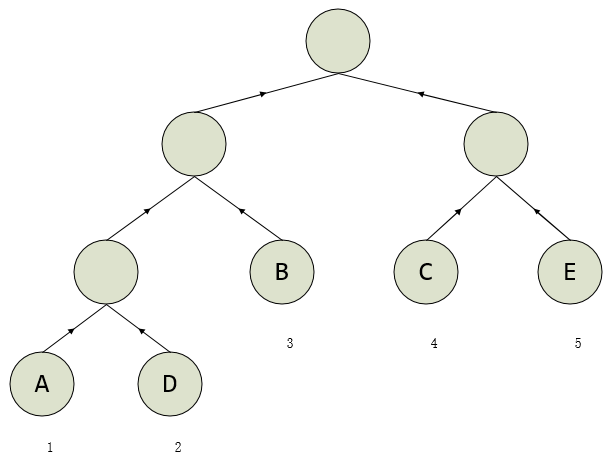
\includegraphics[scale=0.5]{haffmancode.png}
\caption{哈夫曼树编码的示例}
\end{figure}
\noindent  为什么是编码结果为1(A)*3+2(D)*3+3(B)*2+4(C)*2+5(E)*2,我们可以理解为A为第三层,所有要乘3,那A为什么是第三层的呢,也就是因为包含A的节点被合并了3次。所以\textbf{我们只要在模拟生成编码过程中每次合并就累加两个节点的值,那么最终累加出来的结果就是编码结果}。

还有一个编程技巧涉及到了:\\
  $sum[i][j]$是一个二维数组,我们这是可以采用一个一维数组如$s[n]$,来记录$a[i]$的前几项和,令:\\$$s[i] = \sum\limits_{0 \leqslant i \leqslant i}a[i]$$
  这样当我们想知道$sum[i][j]$,只需要$s[j] - s[i-1]$就可以得到结果了,这个编程技巧经常用,但是我一时忘记它叫什么了,说实在我还想了挺久这个技法叫什么的,实在没想起来,什么时候想起来了在补上吧。\\

\section{形式化描述}
\noindent  给定$n$个堆,每个堆共有$a_{i}$个元素,即构成了$$\{a1,a2,\dots,an\}$$我们定义\textbf{每次合并都是相邻的两个堆},并且定义\textbf{合并两个堆的消耗}为两个堆的和,要确定一个合并顺序,使得\textbf{总消耗}最小。

\section{朴素解法}
\noindent  依次地两两合并,对于n个元素的集合,第一次合并共有n-1种可能,假设我们在$k$处合并,在第一次合并的基础上,左边那堆有$k$种可能,右边那个堆共有$(n-k)$种可能,以此类推,朴素解法的时间复杂度为:
\begin{equation}
T(n) = \left\{
\begin{array}{cc}
0&, n=1\\
\sum\limits_{k=1}^{n-1}T(k)T(n-k)&, n>1\\
\end{array}
\right.
\end{equation}
这个结果与矩阵连乘算法的朴素算法的时间复杂度一致,也就是$Catalan$数,计算开来就是:
\begin{equation}
T(n) = \Omega{
\left(\frac{4^{n}}{n^{3/2}}\right)}
\end{equation}
\noindent  补充一下,这样的合并算法应该是采用DFS去搜吧。(存疑...,可以讨论)。显然这个解法是不可接受的。

\section{动态规划可行性证明}
\noindent  做到这里,我越来越觉得这个题目有点像矩阵连乘问题,我参考着它来证明一下动态规划可行性

\subsection{重叠子问题性质}
\begin{figure}[H]
\centering
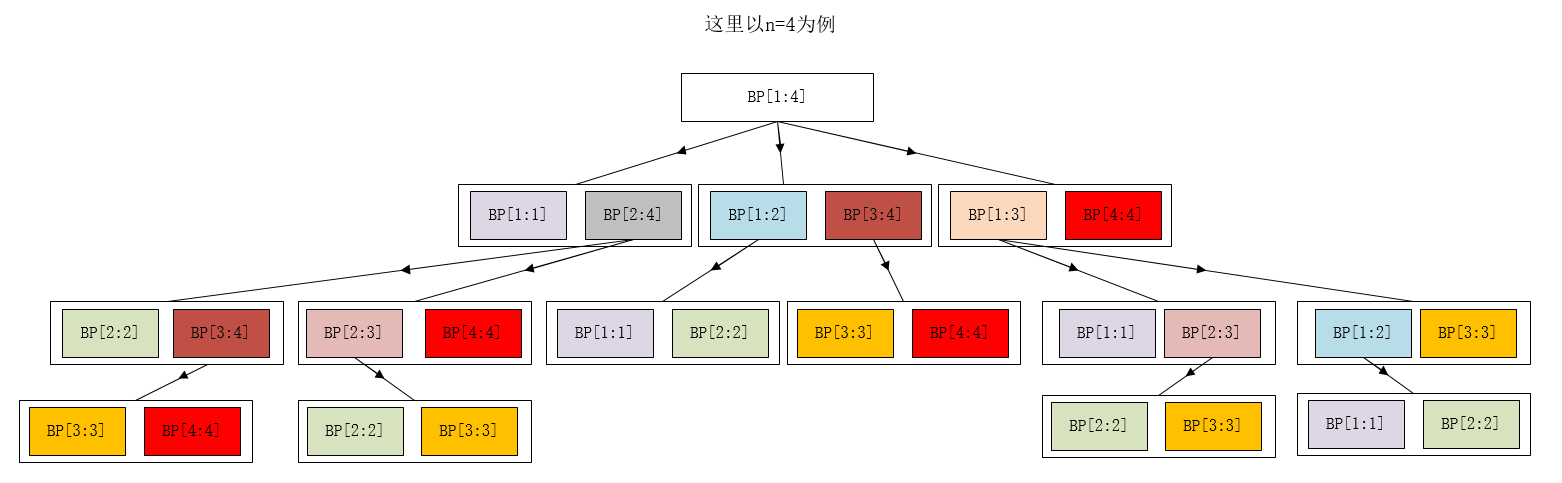
\includegraphics[scale=0.5]{tree.png}
\caption{例:$n=4$时的解递归树}
\end{figure}
\noindent  大家通过递归树,也就可以看出重叠子问题了吧。


\subsection{最优子结构性质}
\noindent  这个问题显然是有最优子结构性质的:\\
  设:$BP[i:j]$表示从i堆到j堆字符所生成的编码结果,并设$BP[i:j]$的最后一次合并子节点在$k$处,则$BP[i:j] \gets BP[i,k] + BP[k+1,j]$\\
  假设:$BP[i:j]$所生成的编码结果是最优的,但是其子结构不是最优的,这里我们假设$BP[i,k]$不是最优子结构\\
  则一定存在一个最优的$BP[i,k]$,当这个最优的$BP[i,k]$加上$BP[k+1,j]$得到的新的$BP[i:j]$显然是优于原来的。\\
  与假设“$BP[i:j]$所生成的编码结果是最优的,但是其子结构不是最优的”矛盾\\
\section{动态规划解法思路}
\noindent  1. 当$i=j$时,$A[i:j]$表示只有一个堆,这样也就不用编码,所以对应的$dp[i][j]=0$\\
  2. 当$i \neq j$时,我们从这几个堆分成两部分,我们假设$k$为那个最佳的合并点,再把这两部分合并,即将$A[i:k]$和$A[k+1:j]$合并,所以对于这种情况$dp[i][j]=dp[i][k]+dp[k+1][j]+sum[i:j]$,当然我们需要用一层循环来找那个最优的$k$点。\\
再提供一下\textbf{递推解结构}:
\begin{equation}
dp[i][j] = \left\{
\begin{array}{cc}
0& ,i=j\\
\min\limits_{i \leqslant k \leqslant j}\{dp[i][j], dp[i][k]+dp[k+1][j]+sum[i:j]\}& ,i \neq j
\end{array}
\right.
\end{equation}

\section{伪代码}
\begin{algorithm}[H]
\caption{求解最优化的编码方式}
\begin{algorithmic}[1] %每行显示行号
\Require $Array$每一堆字母的个数,$n$堆数
\Ensure 最优的编码消耗
\Function {OptimizedEncode}{$Array, n$}
\For{$i = 1 \to n$}
\For{$j = 1 \to n-i$}
\For{$k = j \to i+j$}
\State{$dp[j][i+j] \gets min\{dp[j][i+j], dp[j][k]+dp[k+1][i+k]+s[i+j]-s[j-1]\}$}
\EndFor
\EndFor
\EndFor
\State \Return{$return dp[1][n]$}
\EndFunction
\end{algorithmic}
\end{algorithm}

\section{代码实现}
\begin{lstlisting}[language=C++]
#include <iostream>
#include <stdio.h>
#include <cstring>
#include <malloc.h>
const int MAX = 9999;
#define N 1001
typedef long long LL;
using namespace std;
LL n, a[N], s[N],dp[N][N];

int optimized_encode()
{
    memset(dp, MAX, sizeof(dp));
    for(int i=0;i<=n;i++)
        dp[i][i] = 0;
    for(int r=1;r<=n;r++) 
    {    
        for(int i=1;i+r<=n;i++)
        {
            int j = i+r;         
            for(int k=i;k<=j;k++)
            {
                int temp = dp[i][k] + dp[k+1][j] + s[j] - s[i-1];
                if(dp[i][j] > temp) dp[i][j] = temp;
            }
        }
    }  
    return dp[1][n];
}

int main()
{
    scanf("%d",&n);
    s[0] = 0;
    for(int i=1;i<=n;i++)
    {
        scanf("%d",&a[i]);
        s[i] = s[i-1] + a[i];
    }
    int result = optimized_encode();
    printf("%d\n",result);
    return 0;
}
\end{lstlisting}
\section{复杂度分析}
\noindent  动态规划的题目嘛,好像也没有说明时间复杂度可以分析,三重循环,好像也没有什么可以分析的,$T(n) = O(n^{3})$,空间复杂度也很easy,$S(n) = O(n^{2})$。

\section{后续优化和感想}
\noindent  1. 起始做到一半时,提交时老是报错,我一直以为时$O(n^{3})$的时间复杂度度太大了,导致通不过,所以我查阅了一些资料,所以才能写这一段:一种叫做\textbf{平行四边形优化}的技术,可以用空间换时间,后来发现是自己的第三层循环写错了,导致一部分的测试集没有通过,所以最后我还是以$O(n^{3})$的时间复杂度通过的题目,通过归通过,但是这个算法的确可以但是做完上面那些已将费了我老大劲了,加上我还没有完全掌握\textbf{平行四边形优化},还有,还要写微机的作业呢,我就等以后空了在做优化啦。\\
  2. 谈谈感想吧,说实在的这道题目,对于这道题目做完了我啥感觉有没有,但是对于矩阵连乘问题我有了更深的理解,挺好的吧,确实这道题目跟矩阵连乘实在很像;同时这也让我明白了变治可以省很多精力,同时适当的归类题目,也可以理清思路。
\end{document}
